\documentclass[11pt]{article}
\usepackage[margin=1in]{geometry}\usepackage{amsmath,booktabs,graphicx,url}
\title{Waypoint-to-State/Control Scheduling Comparison}\author{}\date{}
\begin{document}\maketitle
\section*{Methods}
All methods use the same 200 actual LLM predictions and verified RRT references. Independent minimum snap compares each path on its natural clock. Shared clock assigns the expert horizon to the LLM path. Frenet scoring retains minimum-snap references but projects ordered LLM samples onto expert arc length before comparing the full state and control. Guided fit replaces seventh-order minimum snap with linear motion and symmetric constant-acceleration parabolic blends (blend fraction 0.2), then applies the shared clock. The blend construction follows \emph{Computationally Efficient Algorithm to Generate a Waypoints-Based Trajectory for a Quadrotor UAV}; the state/control mapping is consistent with the differential-flatness discussion in \emph{A Comparative Study of Nonlinear MPC and Differential-Flatness-Based Control for Quadrotor Agile Flight}.
\section*{Selected actual prediction}
This case was selected as a moderate example with nonzero $s_u$ and $s_x$ under all four methods, rather than as an extreme-error case. It is sample 105.

RRT verified waypoints: (0.22,0.89), (0.96,1.21), (1.70,1.53), (2.16,2.05), (1.66,2.92), (1.16,3.78).\\
LLM verified waypoints: (0.22,0.89), (0.89,1.23), (1.56,1.56), (1.62,2.24), (1.69,2.92), (1.42,3.35), (1.16,3.78).
\begin{center}\begin{tabular}{lrrrrr}\toprule
Method & $s_u$ & $s_x$ & $q_u$ & $q_x$ & asymptotic radius term [m]\\\midrule
Different clocks & 1.1651 & 0.7485 & 2.3799 & 1.2813 & 20.2188 \\
Shared clock & 1.1557 & 0.6551 & 2.0227 & 1.0569 & 16.8492 \\
Frenet & 1.1042 & 0.6584 & 1.9028 & 1.2247 & 18.2556 \\
Guided shared & 1.2629 & 0.5597 & 1.8772 & 0.6994 & 12.6990 \\
\bottomrule\end{tabular}\end{center}
The last column substitutes each dataset's quantiles into the existing contraction-tube disturbance term. It isolates the quantile-dependent contribution; it is not a measured flight tracking radius. Independent clocks compare different phases and can inflate derivative-derived control error. Shared scheduling aligns the total execution horizon. Frenet alignment removes wall-clock phase from matching. Guided fit limits high-order polynomial oscillation but introduces explicit acceleration changes at its blends.
\begin{figure}[ht]\centering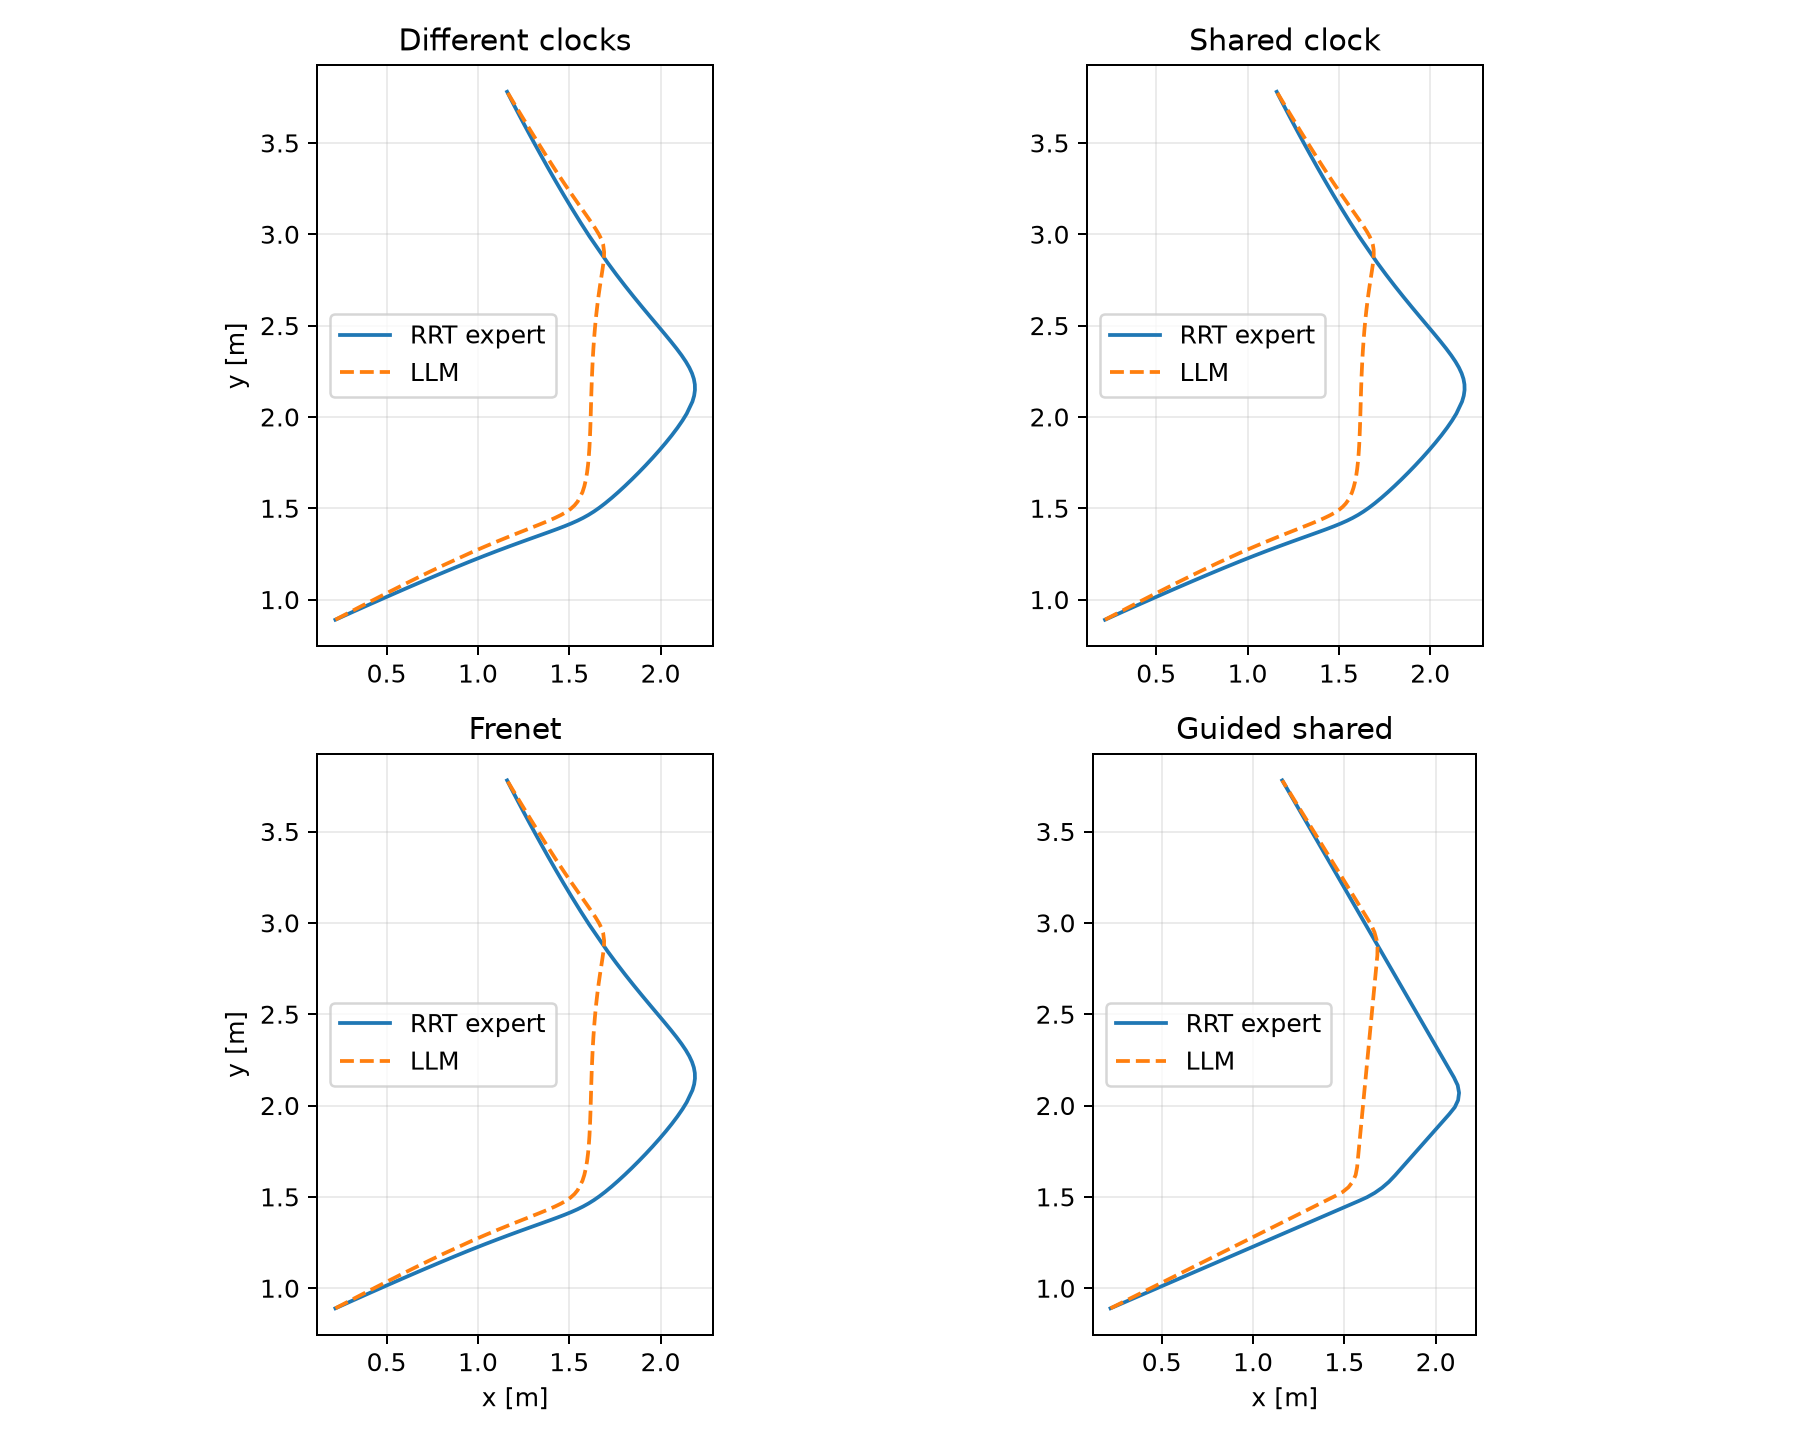
\includegraphics[width=.92\linewidth]{xu_method_comparison_moderate_105_paths.png}\caption{Expert and actual predicted paths.}\end{figure}
\begin{figure}[ht]\centering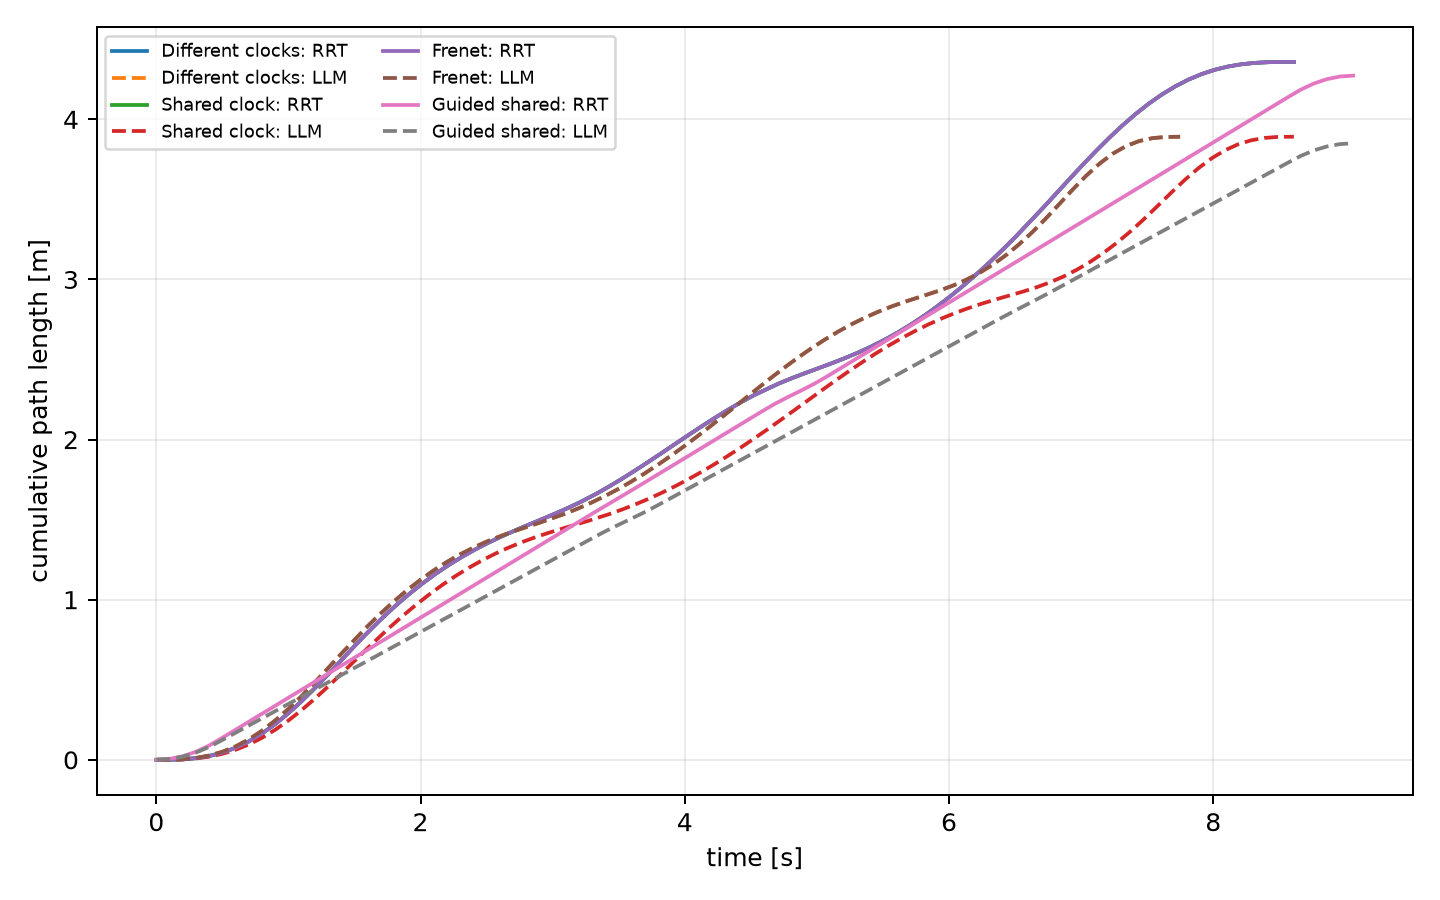
\includegraphics[width=.92\linewidth]{xu_method_comparison_moderate_105_progress.png}\caption{Wall-clock schedule versus spatial progress.}\end{figure}
\begin{figure}[ht]\centering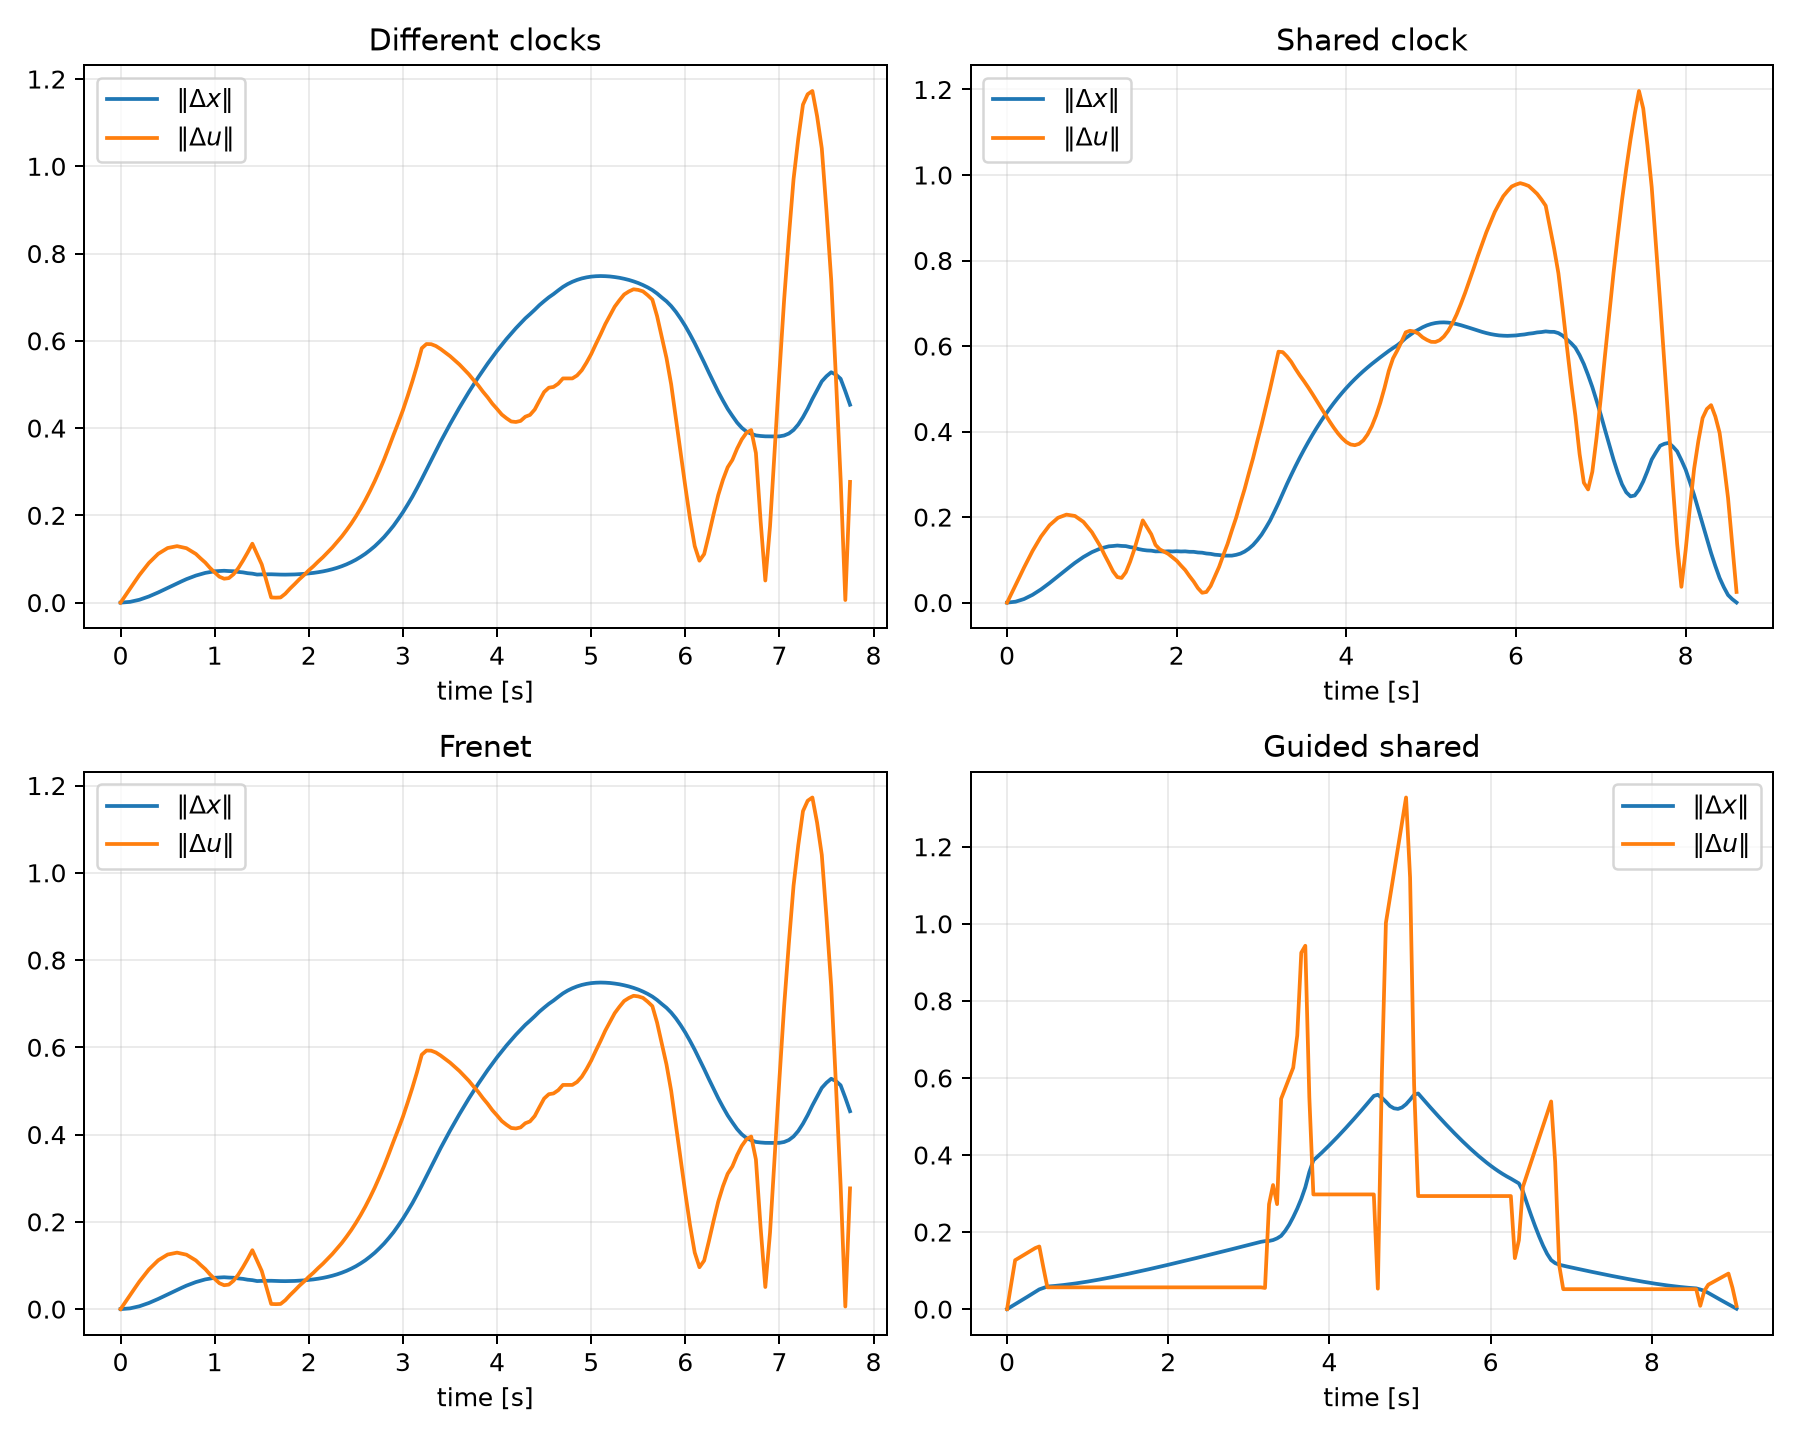
\includegraphics[width=.92\linewidth]{xu_method_comparison_moderate_105_errors.png}\caption{Time-indexed diagnostic state/control errors. Frenet calibration itself uses progress-aligned errors.}\end{figure}
\clearpage\section*{Interpretation}
The numerical comparison separates three causes of large conformal radii: clock phase, spatial disagreement, and trajectory differentiation. Shared scheduling addresses phase at the horizon level; Frenet projection removes phase during scoring; guided parabolic blends avoid seventh-order differentiation. None changes the verified waypoint predictions or the contraction controller.
\end{document}
